\section{Experiments}
\label{sec:Experiments}
\subsection{Experiments Setting}
\noindent \textbf{Implementation Details.} We employ AdamW~\cite{loshchilov2017decoupled} optimizer to train our models. The learning rates are set to \(1e-4\) and \(1e-5\) for SD1.5 and SDXL, respectively. The batch size is set to \(256\), and the total number of training steps is \(50,000\) in the experiment. During the inference phase, we employ the DDIM sampler~\cite{song2020denoising} for the sampling process, configuring it with a total of \(25\) timesteps and a classifier-free guidance scale set to \(7.5\), without the use of negative prompts.

\noindent \textbf{Datasets.} As previously discussed, to align the model with high-quality images across various aesthetic dimensions, we finetune our model using a curated dataset of manually selected images. In the dataset construction phase, we prioritize image quality over quantity. Similar to~\cite{dai2023emu}, we initially extracted \(200k\) images from large, publicly available English datasets such as LAION~\cite{schuhmann2021laion}, employing a combination of automatic and human filtering processes. The automatic filtering included aesthetic scoring, OCR scoring, and CLIP scoring. Human filtering was conducted by individuals with a keen aesthetic sense, adhering to universal photography standards to select the finest images. Furthermore, in addition to the content description texts, we annotate these images with categorical labels across different aesthetic dimensions (such as color, lighting, composition, focus) to serve as additional conditions during our training process.

\noindent \textbf{Evaluation Metrics.} We assess our the performance using the MJHQ-30K dataset~\cite{li2024playground} which contains a large number of high-quality, aesthetically pleasing synthetic data. To enhance our evaluation, we created an additional benchmark, LAION-HQ10K, from the LAION~\cite{schuhmann2021laion} collection, including only high-aesthetic and high-resolution real-word images. This set quantifies the gap between our model's generative capabilities and real-world imagery with exceptional aesthetics. For objective evaluation, we use Fréchet Inception Distance (FID), CLIP Scores, and AES Scores\footnote{https://github.com/christophschuhmann/improved-aesthetic-predictor} to measure the overall quality, fidelity to the original prompts, and aesthetic excellence of the generated images.
% Our evaluation framework encompasses both subjective and objective metrics. 
% \begin{figure*}[ht]
% 	\centerline{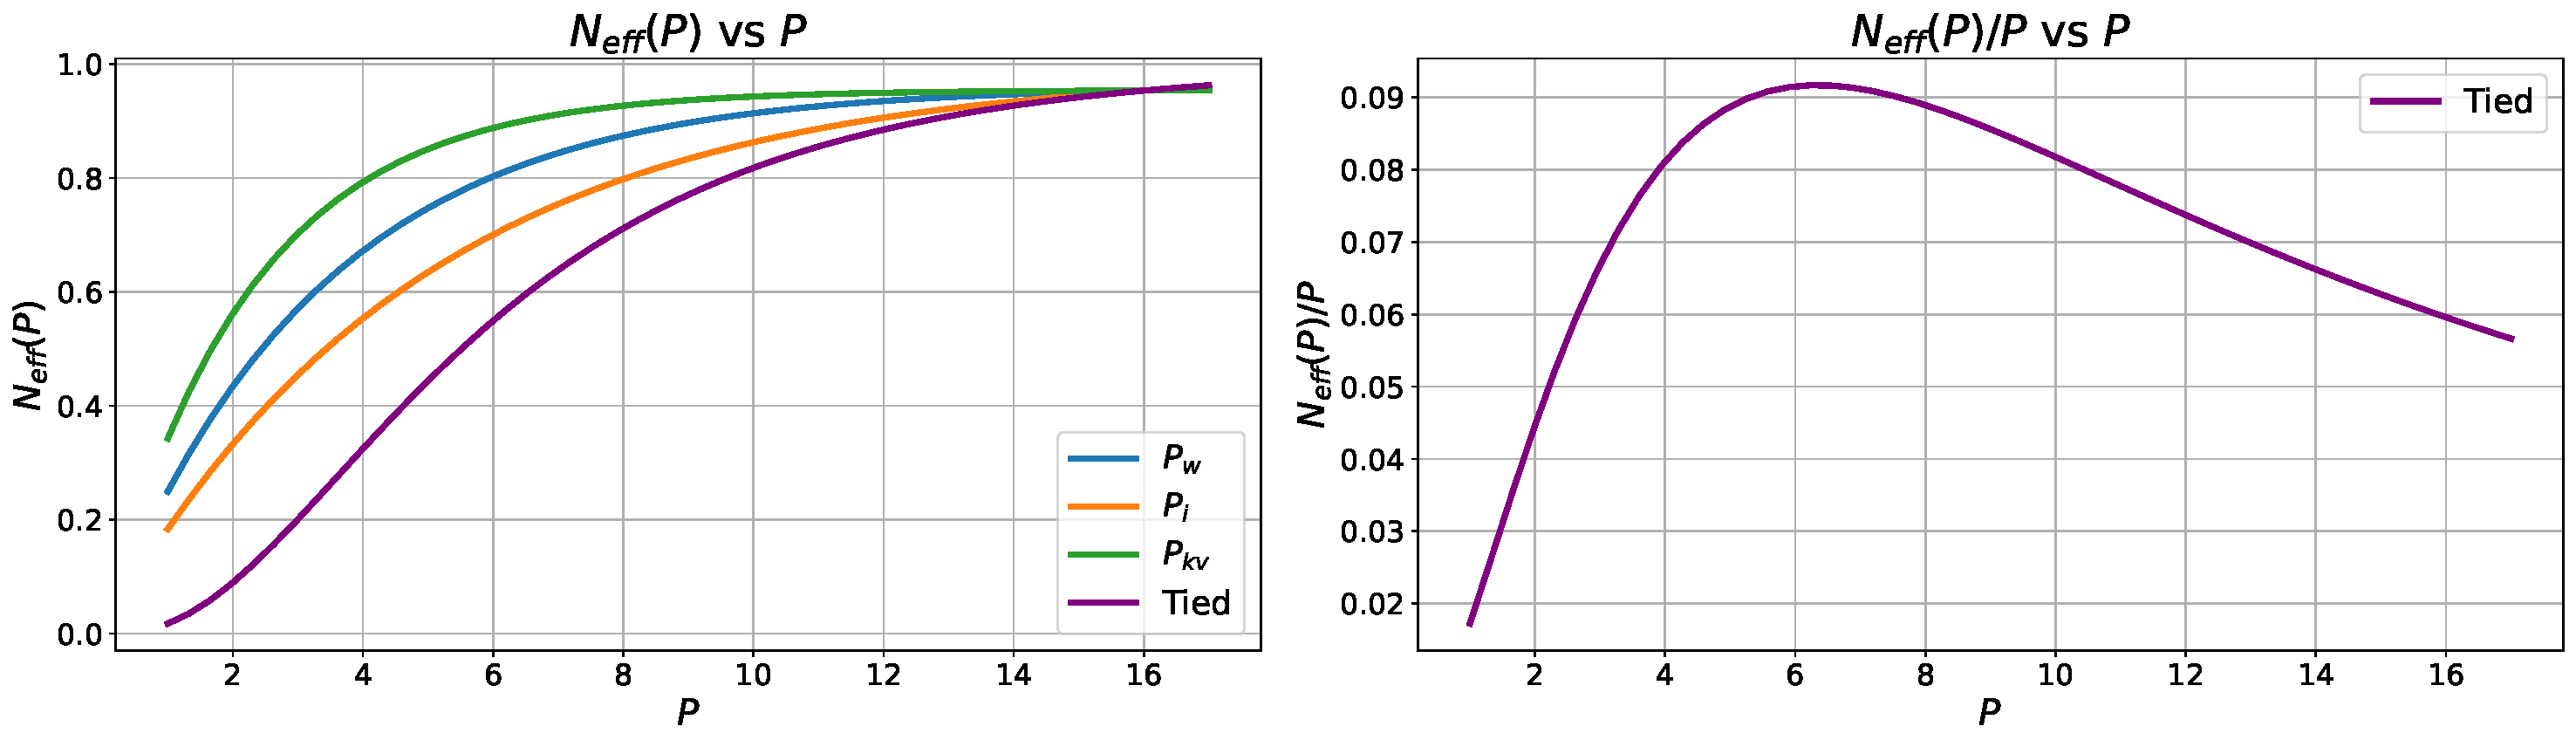
\includegraphics[scale=0.82]{fig6.pdf}}
% 	\caption{Qualitative results. We compare the images generated by VMix and the personalized models. On the left are images produced by the personalized model with VMix integration. On the right are images from the standard personalized model without modifications.}
% 	\label{fig6}
% \end{figure*}

\subsection{Qualitative Analyses}
\noindent \textbf{Compare to other methods.} To validate the effectiveness of VMix, we compared our model to pre-trained model and systematically conducted further comparisons with state-of-the-art methods such as FreeU~\cite{si2023freeu}, DPO~\cite{wallace2024diffusion}, Textual Inversion(TI)~\cite{gal2022image}, and Supervised Fine-Tuning(SFT). We further apply the well-trained VMix model to personalized models, thereby demonstrating the universality of our approach. It should be noted that, to validate the influence of the training set on the generation results, we proceed to utilize SFT and TI for training. In this configuration, the UNet model will be unfrozen, allowing all parameters to be updated. As depicted in Fig.~\ref{fig4} and Fig.~\ref{fig5}, our VMix significantly outperforms other methods in visual appeal, showcasing remarkable aesthetic performance without compromising the image-text alignment capability. In our comparative analysis with Supervised Fine-Tuning (SFT), it became evident that the model struggles with datasets of exceptionally high quality. This difficulty stems from the presence of complex and abstract samples within the dataset that may surpass the model's current capabilities, potentially leading to a decline in performance. VMix mitigates this challenge by incorporating fine-grained aesthetic supervision signals, which streamlines the learning process for the model and, consequently, enhances the overall performance.

\noindent \textbf{Compare to personalized models.} Acting as a versatile plug-and-play adapter, VMix can be directly applied to the personalized model from Civitai\footnote{https://civitai.com}. With the integration of VMix, a notable improvement in the realism and aesthetic appeal of the generated results is expected. See \cref{fig6} for \textit{qualitative results}.

\noindent \textbf{User study.} We further conducted a user study to assess the applicability of VMix as a plug-in. For subjective assessment, 20 evaluators including both aesthetic professionals and non-professionals scored 300 distinct prompts, each yielding 4 generated images. For each case, evaluators need to select the one with the best text fidelity and visual aesthetics from the generation results of the two models. As shown in \cref{fig6}, the results indicate that both pre-trained and open-source models are more favored by users after the application of our VMix method. 

\begin{table}[t]
\centering
\resizebox*{0.425\textwidth}{!}{
\begin{tabular}{lcccc}
\toprule
\textbf{Method} & FID $\downarrow$ & CLIP Score $\uparrow$ & Aes Score $\uparrow$ \\ \hline
SD \cite{rombach2022high} & 28.08 & 30.24 & 5.35 \\
FreeU \cite{si2023freeu} & 27.09 & \textbf{31.00} & 5.36\\
DPO \cite{hu2021lora} &\underline{22.64}  & \underline{30.89} &5.54 \\
Textual Inversion \cite{gal2022image} & 24.72 &  28.92& \underline{5.58}\\
SFT &24.35  & 30.15 & 5.43\\
\hline
\textbf{VMix(Ours)} &\textbf{21.49}  & 30.50 &\textbf{5.79}   \\ \bottomrule
\end{tabular}
}
\caption{Quantitative results on MJHQ-30K benchmark~\cite{li2024playground}. $\uparrow$ stands for higher the better, $\downarrow$ stands for lower the better.}
\label{tab1}
\end{table}

\begin{table}[t]
\centering
\resizebox*{0.425\textwidth}{!}{
\begin{tabular}{lcccc}
\toprule
\textbf{Method} & FID $\downarrow$ & CLIP Score $\uparrow$ & Aes Score $\uparrow$ \\ \hline
SD \cite{rombach2022high} & 25.67 & 32.28 & 5.43 \\
FreeU \cite{si2023freeu} & 28.69 & 32.15 & 5.43\\
DPO \cite{hu2021lora} &\textbf{23.37}  & \underline{32.41} &5.44 \\
Textual Inversion \cite{gal2022image} & 26.62 &  30.97& \underline{5.53}\\
SFT &26.27  & 32.27 & 5.40\\
\hline
\textbf{VMix(Ours)} &\underline{23.92}  & \textbf{32.71} &\textbf{5.68}   \\ \bottomrule
\end{tabular}
}
\caption{Quantitative results on LAION-HQ10K benchmark.}
\label{tab2}
\end{table}

\begin{table}[t]
\centering
\resizebox*{0.425\textwidth}{!}{
\begin{tabular}{lcccc}
\toprule
\textbf{Method} & FID $\downarrow$ & CLIP Score $\uparrow$ & Aes Score $\uparrow$ \\ \hline
Baseline(SD) \cite{rombach2022high} & 28.08 & 30.24 & 5.35 \\ \hline
w/o lora & 21.53 & 30.49 & 5.75\\
w/o vmix &25.64  & 30.16 & 5.52\\
\hline
\textbf{Ours} &\textbf{21.49}  & \textbf{30.50} &\textbf{5.79}   \\ \bottomrule
\end{tabular}
}
\caption{Ablation Study of lora and value-mixed cross-attention. Experiments were conducted on MJHQ-30K benchmark~\cite{li2024playground}.}
\label{tab3}
\end{table}

% \begin{table}[t]
% \centering
% \resizebox*{0.375\textwidth}{!}{
% \begin{tabular}{l|cc}
% \toprule
% \textbf{Model} & \(w/\) VMix  & \(w/o\) VMix  \\ \hline
% SD\cite{rombach2022high} & 84.67\% & 15.33\%  \\
% RealisticVision  & 82.67\% & 17.33\% \\
% Dreamlike &79.67\%  & 20.33\%  \\
% Dreamshaper  & 83.00\% &  17.00\%\\
% \hline
% SDXL~\cite{podell2023sdxl} & 86.33\% & 13.33\%  \\
% AnimeArtXL  & 77.67\% & 22.33\% \\
% LeosamsHelloworldXL &87.33\%  & 12.67\%  \\
% DreamshaperXL  & 85.00\% &  15.00\%\\ \bottomrule
% \end{tabular}
% }
% \caption{The distribution of preferences among human evaluators, showing a dominant inclination towards results with VMix. }
% \label{tab3}
% \end{table}
\begin{figure}
    \centering
    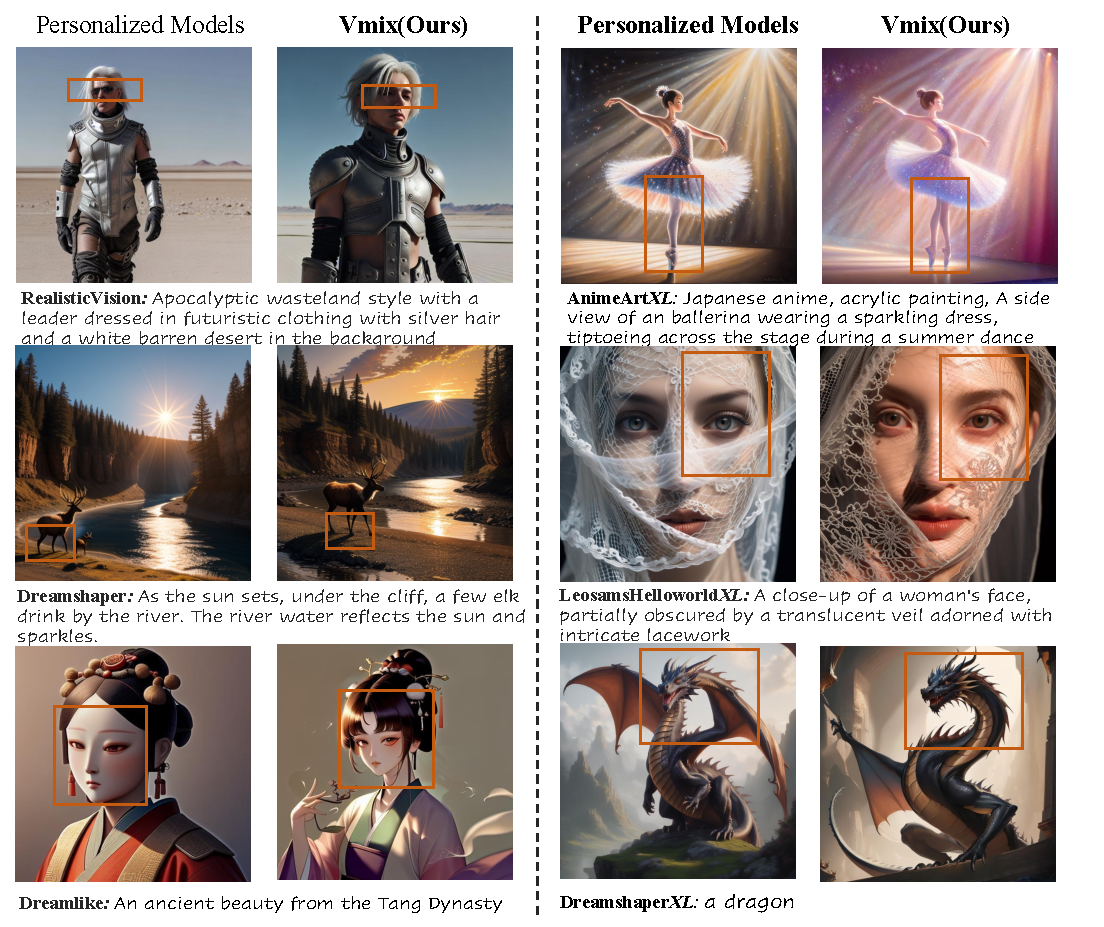
\includegraphics[width=0.88\linewidth]{personal_model_compare.pdf}
    \caption{Qualitative results. We compare images generated by VMix-integrated personalized models with those from standard personalized models. On the left are images produced by the personalized model with VMix integration, while on the right are images from the standard personalized model without modifications.}
    \label{fig6}
\end{figure}

\begin{figure}
    \centering
    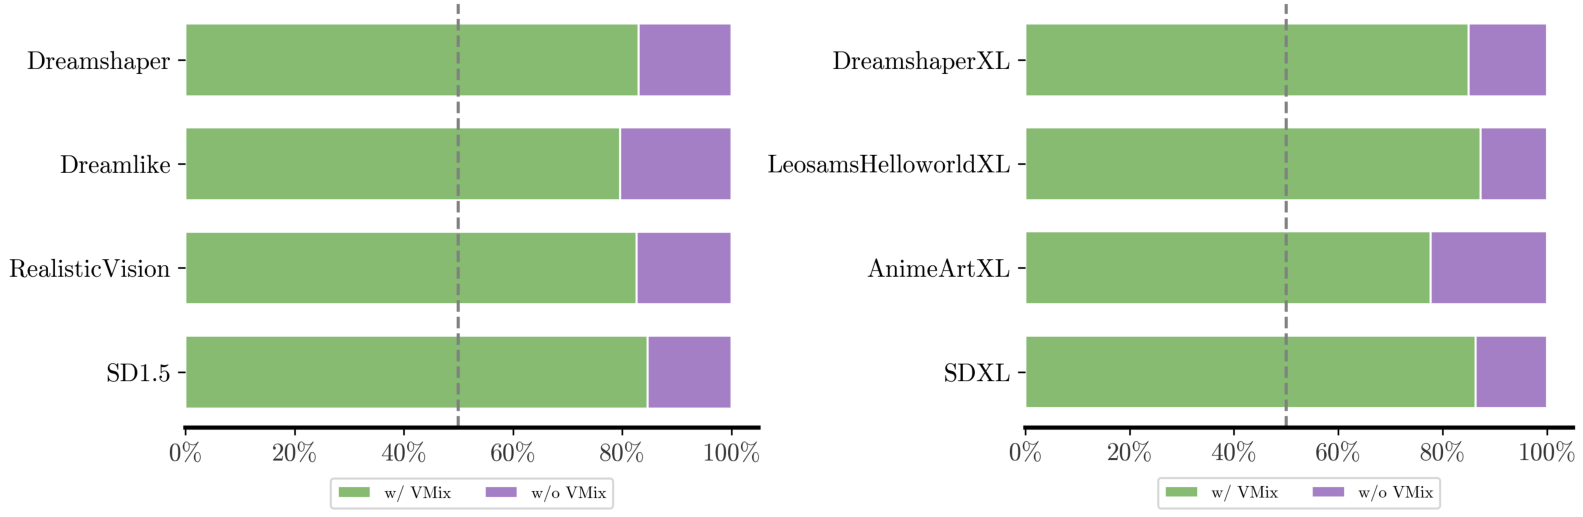
\includegraphics[width=0.85\linewidth]{user_study.pdf}
    \caption{User study. We report the user preference between using VMix and not using VMix.}
    \label{fig7}
\end{figure}

\begin{figure}[ht]
\subfloat[]{
    \begin{minipage}[t]{0.42\linewidth}
        \centering
        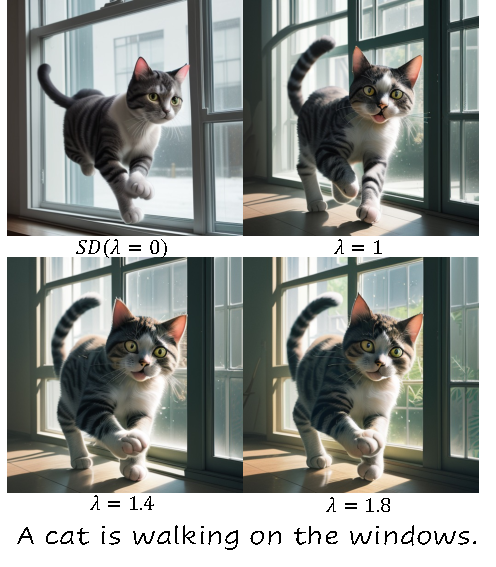
\includegraphics[width=0.88\textwidth]{lambd_cat.pdf}
        % \centerline{(a) PartiPrompts~\cite{yu2022scaling}}
    \end{minipage}}%}
\subfloat[]{
    \begin{minipage}[t]{0.54\linewidth}
        \centering
        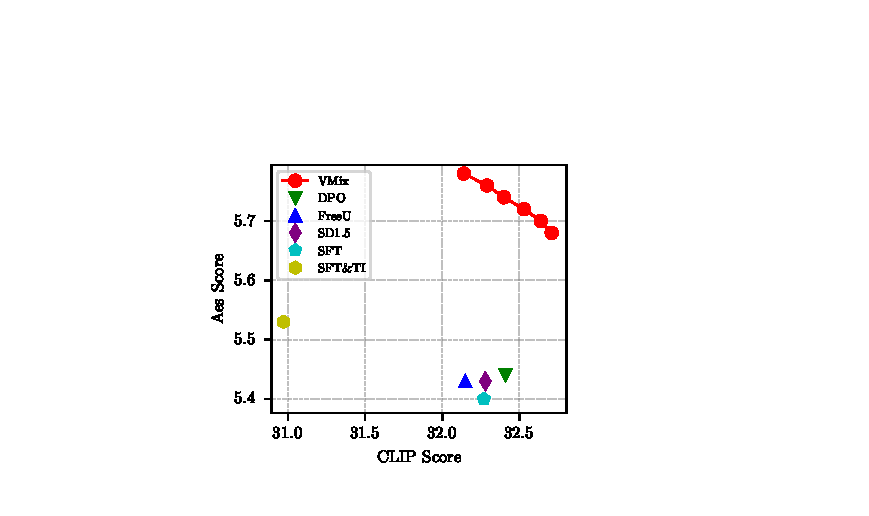
\includegraphics[width=0.85\textwidth]{clip-aes_new.pdf}
        % \centerline{(b)Multi-Category Prompts}
    \end{minipage}}
    \caption{Ablation Study for $\lambda$ of VMix. (a)Visual performance changes of $\lambda$. (b)Performance metrics for VMix, evaluated across a range of $\lambda$ values from 1 to 2 from right to left. }
    \label{fig8}
\end{figure}

% \begin{figure}
%     \centering
%     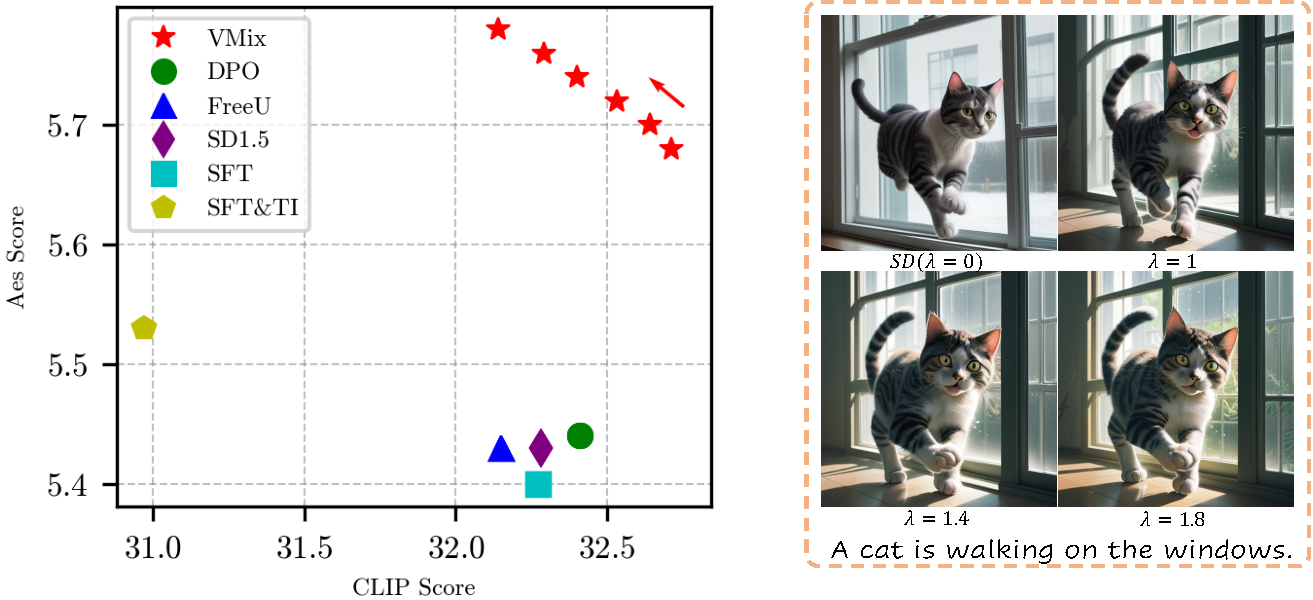
\includegraphics[width=0.8\linewidth]{lambd_fig2.pdf}
%     \caption{Ablation Study for $\lambda$ of VMix. \textit{Left}: performance metrics for VMix, evaluated across a range of $\lambda$ values from 1 to 2. \textit{Right}: visual performance changes of $\lambda$.}
%     \label{fig8}
% \end{figure}

\begin{figure}
    \centering
    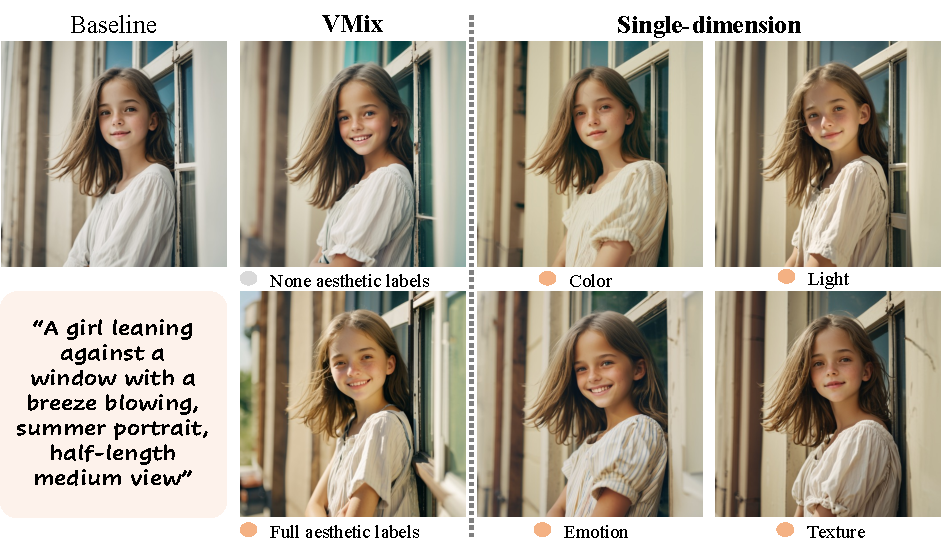
\includegraphics[width=0.88\linewidth]{aes_emb_ab.pdf}
    \caption{Ablation Study for AesEmb of VMix. \textit{Left}: The effects of using all aesthetic labels versus not using them. \textit{Right}: The effects of using single-dimensional aesthetic labels.}
    \label{fig9}
\end{figure}

\subsection{Quantitative Evaluations}
As shown in \cref{tab1} and \cref{tab2}, we have secured the highest Aes Score on both the MJHQ30K and LAION-HQ10K benchmarks, which strongly demonstrates the significance of VMix in enhancing aesthetics. Our performance in CLIP Score and FID metrics is also commendable, indicating that the incorporation of aesthetic embeddings has not detracted from the model's inherent capabilities. Our findings are consistent with the observations made in Figure \ref{fig6}, where VMix significantly enhances the aesthetic dimensions of images, such as lighting and color. Additionally, imperfections on body parts, such as unrealistic limbs or missing extremities, can be further corrected. Moreover, details in close-up images, like skin texture, are also improved, thereby enhancing the overall aesthetic presentation of the images.

\subsection{Ablation Study}
\noindent \textbf{Effect of $\lambda$.} As illustrated in \cref{fig8}, in Value-Mixed Cross-Attention, $\lambda$ is adjustable during inference. When $\lambda$ increases, the Aes Score is observed to gradually increase, while there is a slight decline in the CLIP
Score. However, our method still maintains a significant advantage over other approaches.

\noindent \textbf{Effect of AesEmb.} As illustrated in \cref{fig9}, we conduct an ablation study on the role of AesEmb. When using only single-dimensional aesthetic label, it can be observed that the image quality improves in specific dimensions. When employing full positive aesthetic labels, the visual performance of the images is superior to the baseline overall. This indicates that the incorporation of AesEmb can enhance the visual appearance of images across various aesthetic dimensions. Throughout this process, we did not utilize LoRA.

\noindent \textbf{Effect of LoRA and VMix cross-attention.} In \cref{tab3}, we examine the impact of lora and value-mixed cross-attention utilized in our method. We discover that both of them can enhance the performance metrics of the baseline. Without value-mixed cross-attention, there is a significant drop in the model's performance, with the Aes Score decreasing from $5.79$ to $5.52$ and the CLIP Score from $30.50$ to $30.16$. This indicates that value-mixed cross-attention plays a significant role in text fidelity and image aesthetics. By combining both, we achieved the best performance.
